
%***************************************************************************
%
% CreditCruncher - A portfolio credit risk valorator
% Copyright (C) 2004 Gerard Torrent
%
% This program is free software; you can redistribute it and/or
% modify it under the terms of the GNU General Public License
% as published by the Free Software Foundation; either version 2
% of the License.
%
% This program is distributed in the hope that it will be useful,
% but WITHOUT ANY WARRANTY; without even the implied warranty of
% MERCHANTABILITY or FITNESS FOR A PARTICULAR PURPOSE.  See the
% GNU General Public License for more details.
%
% You should have received a copy of the GNU General Public License
% along with this program; if not, write to the Free Software
% Foundation, Inc., 59 Temple Place - Suite 330, Boston, MA 02111-1307, USA.
%
%
% formulation.tex - TeX documentation file
% --------------------------------------------------------------------------
%
% 2005/01/22 - Gerard Torrent [gerard@fobos.generacio.com]
%   . initial release
%
%***************************************************************************

\chapter{Formulaci\'on del problema}
\label{sec:formulation}

\begin{center}
\framebox{
\begin{minipage}[c]{12.5cm}
Dada una cartera de cr\'editos a empresas de tama\~no mediano, deseamos 
valorar las posibles p\'erdidas debido a los impagos al cabo de un 
tiempo $T$.
\end{minipage}
}
\end{center}

A continuaci\'on se introduce los elementos y propiedades b\'asicas que 
constituyen el marco de trabajo.

%---------------------------------------------------------------------------

\section{Cartera de cr\'editos}

La estructura de la cartera de cr\'editos consiste en un conjunto de
clientes agrupados por sectores de actividad. Cada cliente tiene contratado 
un conjunto de productos de cr\'edito. Cada contrato puede estar 
cubierto por un n\'umero variable de garant\'ias o acuerdos.
Puede verse un esquema de la estructura en la figura \ref{portfolio}.

\begin{figure}[!hb]
\begin{center}
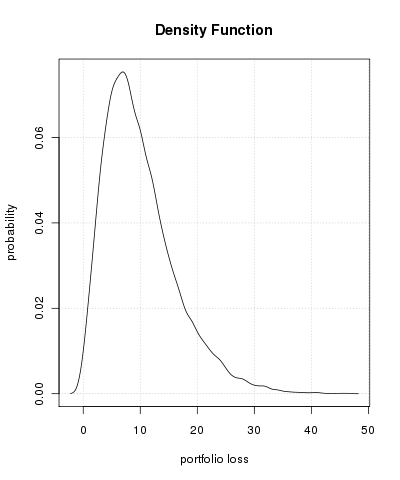
\includegraphics[width=6cm,angle=-90]{./images/portfolio.epsi}
\caption{Estructura de la cartera de cr\'editos}
\label{portfolio}
\end{center}
\end{figure}


\subsection{Ratings}

Un \emph{sistema de ratings}\index{Sistema de ratings} es una medida de calidad
crediticia usada para valorar creditores. A cada creditor se le asigna una nota
discreta (pe. AAA, AA, A, BBB, BB, B, CCC, Default) en funci\'on de su calidad
crediticia. Los \'unicos ratings contemplados en este documento 
son los que tienen una relaci\'on estad\'istica directa y cuantificable 
con la probabilidad de impago del creditor. Ejemplos de este tipo de ratings 
son los publicados por Moody's Investor Service\footnote{http://www.moodys.com} 
o Standard \& Poors\footnote{http://www.standardandpoors.com}. 
\newline
\newline
La metodolog\'ia para la generaci\'on de un sistema de ratings queda fuera del
\'ambito de este documento. CreditCruncher presupone que cada empresa de la 
cartera tiene un rating inicial asignado.
\newline
\newline
El rating de cada empresa puede variar a lo largo del tiempo (v\'ease figura
\ref{ratingevol}). La evoluci\'on temporal del rating de una empresa se
contempla a trav\'es de la matriz de transici\'on o la funci\'on de 
supervivencia (v\'ease la secci\'on \ref{sec:mtransition}).
\begin{figure}[!hb]
\begin{center}
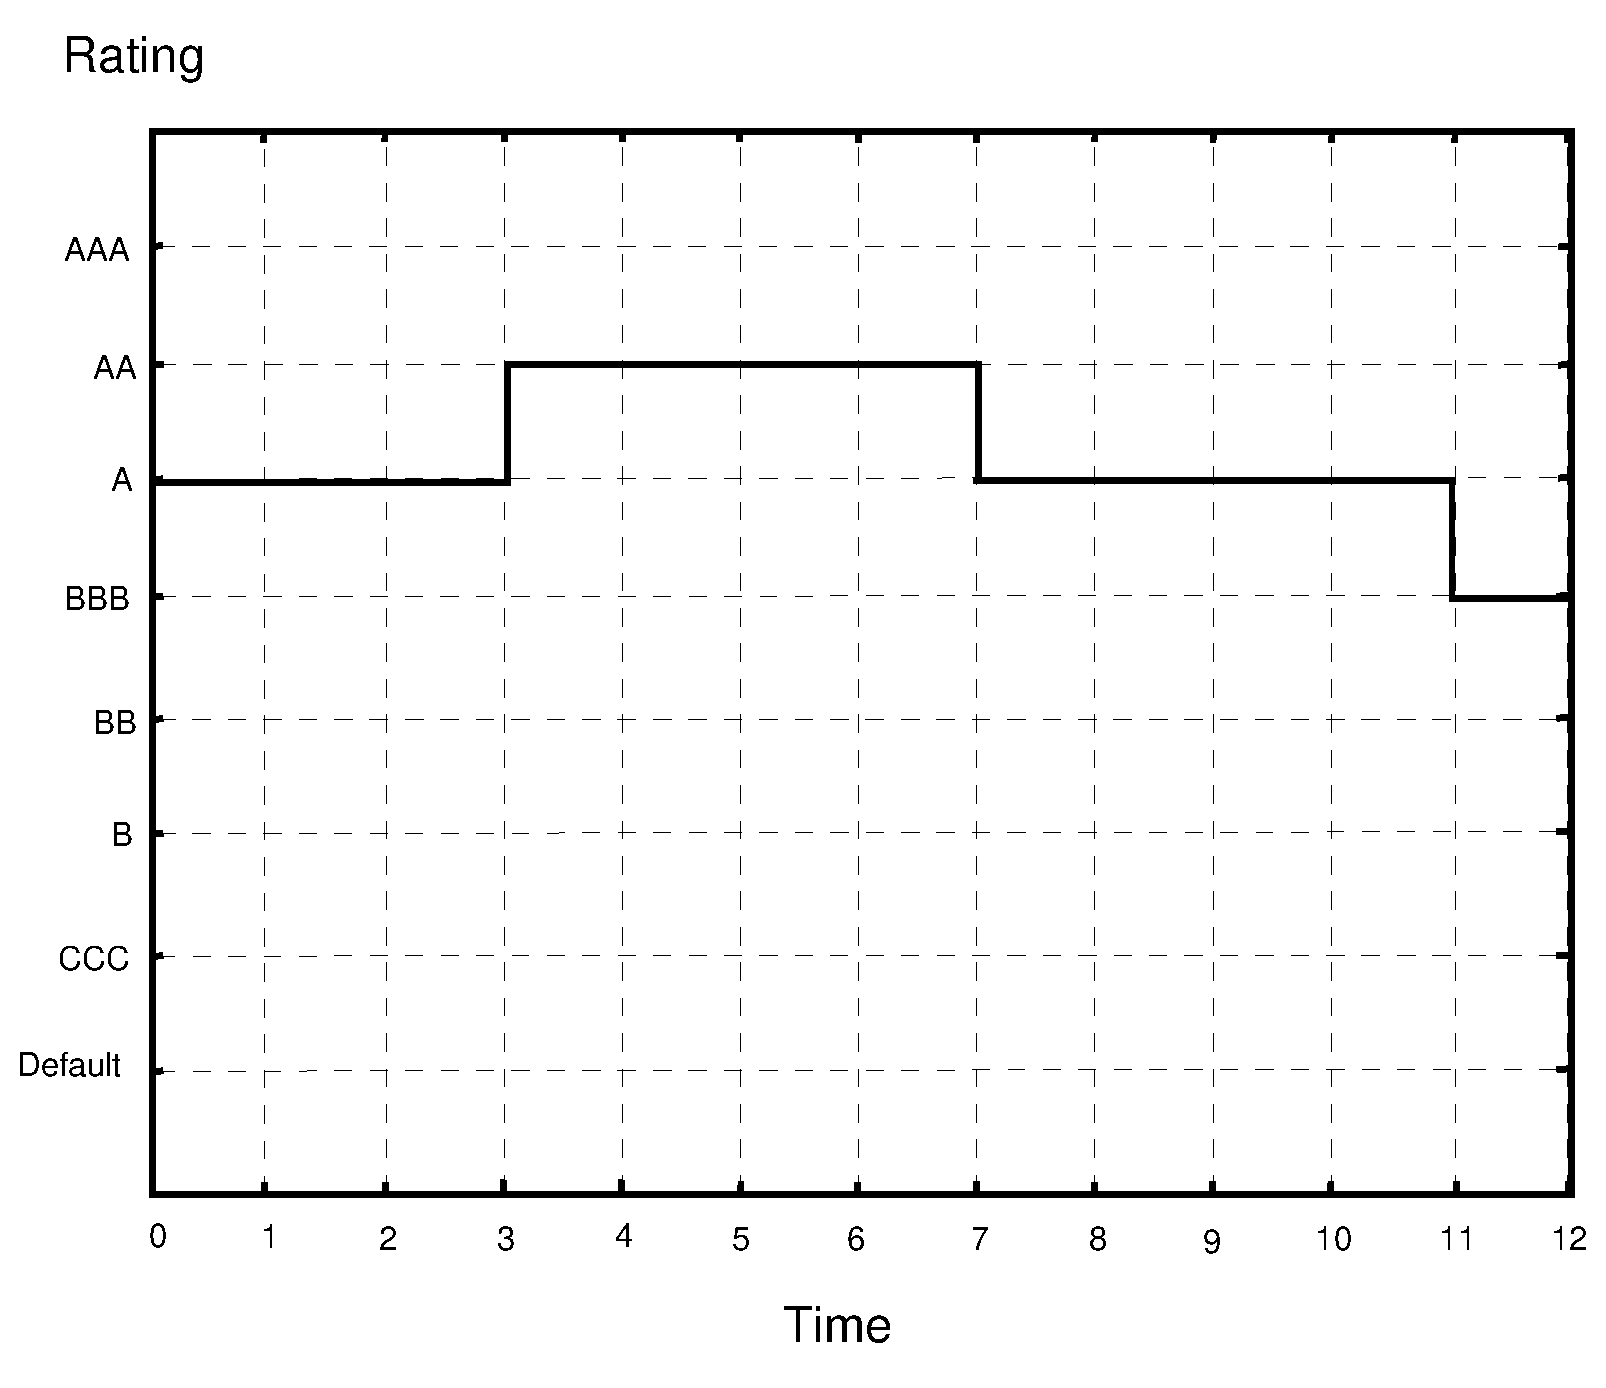
\includegraphics[height=6cm, angle=0]{./images/ratingevol.eps}
\caption{Evoluci\'on del rating a lo largo del tiempo}
\label{ratingevol}
\end{center}
\end{figure}

\paragraph{Notaci\'on.} $P(r_i \to r_j;t_0;t_1) =$ probabilidad de pasar de un 
rating inicial $r_i$ en tiempo $t_0$ a un rating $r_j$ en tiempo $t_1$.


\subsection{Sectores}

La correlaci\'on de fallidos entre clientes es uno de los conceptos que
a\~naden complejidad de la valoraci\'on del riesgo de cr\'edito. No es lo
mismo tener una cartera de cr\'editos donde los clientes hacen fallido 
de forma independiente que una cartera donde los fallidos se encuentran 
correlacionados. En el primer caso, al cabo de un a\~no tendremos un 
conjunto limitado de fallidos. En el segundo caso, al cabo de un a\~no la 
mayoria de clientes habr\'an hecho fallido o casi ning\'un cliente habr\'a
hecho fallido.

\begin{figure}[!hb]
\begin{center}
\includegraphics[width=6cm,angle=-90]{./images/sectorcorrel.ps}
\caption{Impacto de la correlaci\'on intrasectorial}
\label{sectorcorrel}
\end{center}
\end{figure}

Al no poder asignar una correlaci\'on de fallido cliente a cliente, se recurre
a la agrupaci\'on de estos en \emph{sectores}\index{Sectores}. Se considera que
la cartera de cr\'editos dispone de un conjunto de sectores donde los componentes
de cada sector muestran una evoluci\'on crediticia similar. O sea, que la mejora
o empeoramiento de la calidad crediticia (rating) afecta de forma com\'un a los
componentes del sector. En general se identifican estos sectores con los 
sectores industriales. 
\newline
\newline
Se considera que cada cliente pertenece a un \'unico sector y permanece en 
el a lo largo del tiempo. La relaci\'on entre sectores se contempla a trav\'es 
de la matriz de correlaci\'on sectorial (v\'ease la secci\'on \ref{sec:mcorrel}).

\subsection{Activos}

Cada cliente tiene contratado un conjunto de activos con riesgo de cr\'edito.
Caracterizamos un activos por los siguientes elementos (importes positivos
significan que el cliente paga, importes negativos significan que el cliente 
cobra):

\paragraph{Cashflow.} \index{Cashflow} Entregas y devoluciones de dinero a lo largo
del tiempo. Incluye las posibles amortizaciones, primas, cupones, comisiones, costes,
etc. Usaremos el cashflow para calcular el valor, o precio, de un activo en el
instante $t$.

\paragraph{Netting.} \index{Netting} Importe correpondiente a la liquidaci\'on de
deudas mutuas en caso de fallido. Incluye la posible recuperaci\'on, pago de
obligaciones contraidas (pe. en el caso de avales, etc.).

\paragraph{Ejemplo.}
Caracterizamos un bono (bond) de $100$ \euro de valor nominal, con fecha emisi\'on
31/12/2006, tipo de inter\'es anual del $4\%$, pago anual de cupones y amortizaci\'on
al cabo de $5$ a\~nos. En caso de fallido se estima que se recupera un $80\%$ del
importe pendiente de abonar.\newline

\begin{center}
\begin{tabular}{c|r|r}
\textbf{Date} & \textbf{Cashflow} & \textbf{Netting} \\
\hline
31/12/2006 &  -100.00 &    0.00 \\
31/12/2007 &     4.00 &   96.00 \\
31/12/2008 &     4.00 &   92.00 \\
31/12/2009 &     4.00 &   89.60 \\
31/12/2010 &     4.00 &   86.40 \\
31/12/2011 &   104.00 &   83.20
\end{tabular}
\end{center}

\paragraph{Ejemplo.}
Caracterizamos un pr\'estamo hipotecario (mortgage) de $100$ \euro, con fecha
de contrataci\'on 15/01/2006, tipo de inter\'es anual del $6.5\%$ y cuota
(instalment) mensual y un plazo de $25$ a\~nos. La vivienda hipotecada est\'a
valorada en $80$ \euro. Determinamos la cuota mensual usando la siguiente
f\'ormula (canon vencido o m\'etodo franc\'es):
\begin{displaymath}
I =
\frac{A \cdot r \cdot (1+r)^t}{(1+r)^t - 1} =
\frac{100 \cdot (6.5\%/12) \cdot (1+6.5\%/12)^{25\cdot12}}{(1+6.5\%/12)^{25\cdot12} - 1} =
0.67521
\end{displaymath}

\begin{center}
\begin{tabular}{c|r|r}
\textbf{Date} & \textbf{Cashflow} & \textbf{Netting} \\
\hline
15/01/2006 &  -100.00 &    0.00 \\
15/02/2006 &     0.68 &   80.00 \\
15/03/2006 &     0.68 &   80.00 \\
15/04/2006 &     0.68 &   80.00 \\
\dots      &    \dots &   \dots \\
15/11/2030 &     0.68 &   80.00 \\
15/12/2030 &     0.68 &   80.00 \\
15/01/2031 &     0.68 &   80.00
\end{tabular}
\end{center}

\paragraph{Ejemplo.}
Caracterizamos un aval (endorsement) por un importe avalado de $100$ \euro
con fecha de contrataci\'on 15/01/2006, durante un periodo de $2$ a\~nos y
una cuota semestral anticipada de $4.5$ \euro.

\begin{center}
\begin{tabular}{c|r|r}
\textbf{Date} & \textbf{Cashflow} & \textbf{Netting} \\
\hline
15/01/2006 &     4.50 &    0.00 \\
15/07/2006 &     4.50 & -100.00 \\
15/01/2007 &     4.50 & -100.00 \\
15/07/2007 &     4.50 & -100.00 \\
15/01/2008 &     0.00 & -100.00
\end{tabular}
\end{center}


%---------------------------------------------------------------------------

\section{Tipos de inter\'es}
\label{sec:interests}

\paragraph{Definici\'on.}
Sea $C_{t_0}$ el importe inicial de una operaci\'on y $C_{t_1}$ el importe final. 
Definimos el \emph{tipo de inter\'es efectivo}\index{Tipo de inter\'es efectivo},$r$,
como:
\begin{equation}
C_{t_1} = C_{t_0} \cdot (1+r)
\end{equation}

\begin{equation}
\label{tipus_efectiu}
r = \frac{C_{t_1}-C_{t_0}}{C_{t_0}}
\end{equation}

\paragraph{Definici\'on.}
El \emph{tipo de inter\'es simple}\index{Tipo de inter\'es simple}, $r_s$, es un tipo
de inter\'es donde para cada periodo de tiempo se incrementa el importe inicial, $C_{t_0}$
por un factor de $r_s$.
\begin{equation}
C_{t_1} = C_{t_0} \cdot (1+ r_s \cdot (t_1-t_0))
\end{equation}

\begin{equation}
\label{interes_simple_1}
r_s = \frac{r}{t_1 - t_0}
\end{equation}

\paragraph{Defici\'on.}
El \emph{tipo de inter\'es compuesto}\index{Tipo de inter\'es compuesto}, $r_c$, es un tipo
de inter\'es donde en cada periodo de tiempo se incrementa por un factor de $r_c$ el importe
acumulado del periodo anterior.
\begin{equation}
C_{t_1} = C_{t_0} \cdot (1+ r_c)^{(t_1-t_0)} 
\end{equation}

\begin{equation}
\label{interes_compuesto_1}
r_c = (1 + r) ^ \frac{1}{t_1-t_0} - 1
\end{equation}

\paragraph{Defici\'on.}
El \emph{tipo de inter\'es continuo}\index{Tipo de inter\'es continuo}, $r_e$, es el caso
l\'\i mite del inter\'es compuesto.
\begin{equation}
C_{t_1} = C_{t_0} \cdot e^{r_e \cdot (t_1-t_0)}
\end{equation}

\begin{equation}
\label{interes_continuo_2}
r_e = \ln(1 + r_c)
\end{equation}

La f\'ormula exponencial, no el coeficiente, se obteniene considerando el
l\'\i mite del tipo de inter\'es compuesto.
\begin{equation}
\label{interes_continuo_1}
\begin{array}{c}
\lim_{t_1 \rightarrow t_0} 1+r_c = 
\lim_{t_1 \rightarrow t_0} (1 + r)^{\frac{1}{t_1 - t_0}} = \cr
\lim_{t_1 \rightarrow t_0} (1 + r_s \cdot (t_1-t_0)) ^ {\frac{1}{t_1 - t_0}} =
\lim_{n \rightarrow \infty} (1 + \frac{r_s}{n}) ^ {n} = 
e^{r_s}
\end{array}
\end{equation}

\paragraph{Ejemplo.}
Consideremos una operaci\'on que supone una inversi\'on inicial de 100 MM. y que 
al cabo de 5 a\~{n}os proporciona unos ingresos de 120 MM. 
\newline
\newline
Calculemos los diferentes tipos de inter\'es:
\begin{displaymath}
\begin{array}{l}
r = \frac{120-100}{100} = 20 \% \cr
r_s= \frac{r}{5} = \frac{20 \%}{5} = 4 \% \cr
r_c= (1+r) ^ {1/5} - 1 = 1.2^{0.2} - 1 = 1.0371 - 1 = 3.71 \% \cr
r_e= \ln(1 + r_c) = \ln(1.0371) = 3.65 \%
\end{array}
\end{displaymath}
\newline
\newline
Recuperemos el importe final de la operaci\'on a partir del importe inicial, 
el intervalo de tiempo y el tipo de inter\'es:
\begin{displaymath}
\begin{array}{lcl}
\textrm{tipo efectivo}       & \rightarrow & C_{t_1} = 100 \cdot (1 + 20\%) = 120 \cr
\textrm{inter\'es simple}    & \rightarrow & C_{t_1} = 100 \cdot (1 + 4\% \cdot 5) = 120 \cr
\textrm{inter\'es compuesto} & \rightarrow & C_{t_1} = 100 \cdot (1 + 3.71\%)^5 = 120 \cr
\textrm{inter\'es continuo}  & \rightarrow & C_{t_1} = 100 \cdot e^{3.65 \% \cdot 5} = 120
\end{array}
\end{displaymath}

\subsection{Funci\'on de transporte}

\paragraph{Definici\'on.} Fijado un tipo de inter\'es, $r$, y un intervalo de
tiempo, $\Delta t = t_k-t_0$, \emph{la funci\'on de transporte}\index{Funci\'on de transporte},
$\Upsilon$, proporciona el factor que debe aplicarse a un importe en $t_0$ para obtener el
importe equivalente en $t_k$.
\newline
\newline
Caso $C_0 \longrightarrow C_k \quad t_0 < t_k$:
\begin{displaymath}
\begin{array}{lcl}
\textrm{inter\'es simple}    & \rightarrow & C_0 \cdot \Upsilon(t_0,t_k, r) = C_0 \cdot (1+r\cdot(t_k-t_0)) = C_k \cr
\textrm{inter\'es compuesto} & \rightarrow & C_0 \cdot \Upsilon(t_0,t_k, r) = C_0 \cdot (1+r)^{(t_k-t_0)} = C_k \cr
\textrm{inter\'es continuo}  & \rightarrow & C_0 \cdot \Upsilon(t_0,t_k, r) = C_0 \cdot e^{r\cdot(t_k-t_0)} = C_k 
\end{array}
\end{displaymath}
Caso $C_k \longleftarrow C_0 \quad t_k < t_0$:
\begin{displaymath}
\begin{array}{lcl}
\textrm{inter\'es simple}    & \rightarrow & C_0 \cdot \Upsilon(t_0,t_k, r) = C_0 \cdot (1+r\cdot(t_0-t_k))^{-1} = C_k \cr
\textrm{inter\'es compuesto} & \rightarrow & C_0 \cdot \Upsilon(t_0,t_k, r) = C_0 \cdot (1+r)^{-(t_0-t_k)} = C_k \cr
\textrm{inter\'es continuo}  & \rightarrow & C_0 \cdot \Upsilon(t_0,t_k, r) = C_0 \cdot e^{-r\cdot(t_0-t_k)} = C_k
\end{array}
\end{displaymath}

\paragraph{Notaci\'on.} En este documento se considera que el tipo de inter\'es
aplicado es el tipo de inter\'es compuesto. En este caso, la funci\'on de transporte
tiene una expresi\'on \'unica, sea cual sea el sentido en el que se aplica:
\begin{displaymath}
\Upsilon(t_0,t_k, r) = (1+r)^{(t_k-t_0)}
\end{displaymath}


\subsection{Curva spot o cup\'on cero}

\paragraph{Definici\'on.} La \emph{curva spot}\index{Curva spot} o
\emph{curva cup\'on cero}\index{Curva cup\'on cero} es la funci\'on
$S$ que indica el tipo de inter\'es a aplicar en la funci\'on de transporte
desde el tiempo $t_0$.

En el mercado existen productos simples a distintos plazos para los cuales se 
puede calcular el tipo de inter\'es que proporcionan. Estos tipos de inter\'es
solamente se pueden usar en la funci\'on de transporte cuando uno de los
tiempos sea $t_0$ y el otro sea superior a $t_0$.

\begin{figure}[!hb]
\begin{center}
\includegraphics[height=10cm, angle=-90]{./images/spot.ps}
\caption{Curva Spot}
\label{spot}
\end{center}
\end{figure}

\paragraph{Proposici\'on.} Dada una curva spot $S_{t_0}$ en $t_0$, podemos calcular
el coeficiente de transporte para todo $t_i, t_j \ge t_0$:
\begin{displaymath}
\Upsilon(t_i,t_j, r) = 
\Upsilon(t_i,t_0, S_{t_o}(t_i)) \cdot \Upsilon(t_0,t_j, S_{t_0}(t_j))
\end{displaymath}


%---------------------------------------------------------------------------

\section{Matriz de transici\'on}
\label{sec:mtransition}

\paragraph{Definici\'on.} La \emph{matriz de transici\'on}\index{Matriz de transici\'on}
en el periodo $T$ es una matriz cuadrada que proporciona la probabilidad que un cliente
con rating inicial $r_i$ pase a tener, al cabo de un tiempo $T$, rating $r_j$.
La denotamos de la forma siguiente:
\begin{displaymath}
M_T = \left(
\begin{array}{ccc}
m_{1,1} & \dots  & m_{1,n} \cr
\vdots & \ddots & \vdots \cr
m_{n,1} & \dots  & m_{n,n} 
\end{array}
\right)
\qquad
m_{i,j} = P(r_i \to r_j;0;T)
\end{displaymath}

donde $n$ es el n\'umero de ratings y $m_{i,j}$ corresponde a la probabilidad de que un
cliente con rating $r_i$ pase a tener, al cabo de $T$ tiempo, rating $r_j$.

\paragraph{Ejemplo.} Matriz de transici\'on anual ($T=1$ a\~no).
Las probabilidades est\'an expresadas en tanto por ciento.
\\
\begin{center}
\begin{tabular}[]{l|rrrrrrrr}
        &      AAA &       AA &        A &      BBB &       BB &        B &      CCC &  Default \cr
\hline
AAA     &  $90.81$ &   $8.33$ &   $0.68$ &   $0.06$ &   $0.12$ &   $0.00$ &   $0.00$ &   $0.00$ \cr
 AA     &   $0.70$ &  $90.65$ &   $7.79$ &   $0.64$ &   $0.06$ &   $0.14$ &   $0.02$ &   $0.00$ \cr
  A     &   $0.09$ &   $2.27$ &  $91.05$ &   $5.52$ &   $0.74$ &   $0.26$ &   $0.01$ &   $0.06$ \cr
BBB     &   $0.02$ &   $0.33$ &   $5.95$ &  $86.93$ &   $5.30$ &   $1.17$ &   $0.12$ &   $0.18$ \cr
 BB     &   $0.03$ &   $0.14$ &   $0.67$ &   $7.73$ &  $80.53$ &   $8.84$ &   $1.00$ &   $1.06$ \cr
  B     &   $0.00$ &   $0.11$ &   $0.24$ &   $0.43$ &   $6.48$ &  $83.46$ &   $4.07$ &   $5.21$ \cr
CCC     &   $0.22$ &   $0.00$ &   $0.22$ &   $1.30$ &   $2.38$ &  $11.24$ &  $64.86$ &  $19.78$ \cr
Default &   $0.00$ &   $0.00$ &   $0.00$ &   $0.00$ &   $0.00$ &   $0.00$ &   $0.00$ & $100.00$
\end{tabular}
\end{center}
En particular, la probabilidad que un cliente con rating $AA$ pase a tener 
rating $B$ al cabo de $1$ a\~no es del $0.14\%$.

\subsection{Propiedades}

\paragraph{Propiedad 1.}
El valor de los elementos de la matriz de transici\'on se encuentran entre $0$ 
y $1$ debido a que los elementos de la matriz son probabilidades.

\begin{displaymath}
0 \leq m_{i,j} \leq 1 \quad \forall i,j
\end{displaymath}

\paragraph{Propiedad 2.}
La suma de los elementos de cualquier fila de la matriz de transici\'on suman $1$.
De esta forma se  est\'a imponiendo que el conjunto de ratings finales solo puede 
ser el de los ratings contemplados en la matriz.

\begin{displaymath}
\sum_{j=1}^{n} m_{i,j} = 1 \quad \forall i
\end{displaymath}

\paragraph{Propiedad 3.}
Los elementos de la fila correspondiente al rating $Default$ ($r_n$), son todos 
$0$, excepto el elemento de la columna que corresponde al rating $Default$, 
$m_{n,n}$, que vale $1$. Esta condici\'on indica que cuando se llega al estado 
de fallido no es posible salir de este estado.

\begin{displaymath}
\begin{array}{ll}
m_{n,j} = 0        & \quad \forall j \neq n \cr
m_{n,n} = 1
\end{array}
\end{displaymath}

\paragraph{Propiedad 4.}
Sea cual sea el rating inicial, existe la posibilidad que realize fallido.

\begin{displaymath}
\forall i \quad \exists j \quad \textrm{tq.} \quad m_{i,j} > 0 \quad \textrm{and} \quad  m_{j,n} > 0
\end{displaymath}


\subsection{Cambio de periodo}

Deseamos obtener la matriz de transici\'on para periodos distintos (m\'ultiplos o 
fraccionarios) del periodo proporcionado, $T$. Esto nos permitir\'a determinar la 
probabilidad que un cliente con rating inicial $r_i$ tenga rating $r_j$ al cabo 
de $k \cdot T$ tiempo o al cabo de $T/k$ tiempo.

\paragraph{Ejemplo.} Calculemos la probabilidad de pasar de rating $AA$ a
rating $B$ en un plazo de dos a\~nos disponiendo de la matriz de transici\'on anual.

\begin{displaymath}
\begin{array}{llll}
P(AA \to B;0;2) = & P(AA \to AAA;0;1)     & \cdot P(AAA \to B;1;2)     & + \cr
                  & P(AA \to AA;0;1)      & \cdot P(AA \to B;1;2)      & + \cr
                  & P(AA \to A;0;1)       & \cdot P(A \to B;1;2)       & + \cr
                  & P(AA \to BBB;0;1)     & \cdot P(BBB \to B;1;2)     & + \cr
                  & P(AA \to BB;0;1)      & \cdot P(BB \to B;1;2)      & + \cr
                  & P(AA \to B;0;1)       & \cdot P(B \to B;1;2)       & + \cr
                  & P(AA \to CCC;0;1)     & \cdot P(CCC \to B;1;2)     & + \cr
                  & P(AA \to Default;0;1) & \cdot P(Default \to B;1;2) &
\end{array}
\end{displaymath}

Notamos que se trata del producto de la fila correspondiente al rating $AA$ 
(rating de salida) por la columna correspondiente al rating $B$ (rating de 
llegada).

\paragraph{Proposici\'on.} Sean $M_{T_1}$ y $M_{T_2}$ las matrices de transici\'on
para los periodos $T_1$ y $T_2$. Entonces, la matriz de transici\'on para el
periodo $T_1+T_2$ es:
\begin{displaymath}
M_{T_1+T_2} = M_{T_1} \cdot M_{T_2}
\end{displaymath}

\paragraph{Corolario.} Sean $M_{T}$ la matriz de transici\'on para el periodo 
$T$ y $k \in \mathrm{N}$. Entonces\footnote{v\'ease el ap\'endice \ref{apendix:sqrtmat} 
para ver como se calcula la ra\'iz de una matriz}:
\begin{displaymath}
M_{k \cdot T} = M_{T}^k
\end{displaymath}
\begin{displaymath}
M_{\frac{T}{k}} = \sqrt[k]{M_{T}}
\end{displaymath}


\subsection{Funci\'on de supervivencia}

\paragraph{Definici\'on.} La \emph{Tasa de Morosidad Anticipada}
\index{Tasa de Morosidad Anticipada} (TMA) del rating $r_i$ en el a\~no $k$ es
la probabilidad que una empresa con rating inicial $r_i$ haga fallido a lo largo
del a\~no $k$.

\begin{figure}[!hb]
\begin{center}
\includegraphics[height=10cm, angle=-90]{./images/tma.ps}
\caption{Tasa de Morosidad Anticipada}
\label{tma}
\end{center}
\end{figure}

\paragraph{Definici\'on.} La \emph{Tasa de Morosidad Anticipada Acumulada}
\index{Tasa de Morosidad Anticipada Acumulada} (TMAA) del rating $r_i$ en el
tiempo $t$ es la probabilidad que una empresa con rating inicial $r_i$ haga
fallido en el intervalo de tiempo $(0,t)$.

\begin{displaymath}
TMAA(r_i,t)=P(r_i \to Default;0;t)
\end{displaymath}

\begin{figure}[!hb]
\begin{center}
\includegraphics[height=10cm, angle=-90]{./images/tmaa.ps}
\caption{Tasa de Morosidad Anticipada Acumulada}
\label{tmaa}
\end{center}
\end{figure}

\paragraph{Definici\'on.} La \emph{Supervivencia}\index{Supervivencia} en el
tiempo $t$ del rating $r_i$ es la probabilidad que una empresa con rating inicial
$r_i$ no haya hecho fallido en el intervalo de tiempo $(0,t)$.

\begin{figure}[!hb]
\begin{center}
\includegraphics[height=10cm, angle=-90]{./images/survival.ps}
\caption{Funci\'on de Supervivencia}
\label{survival}
\end{center}
\end{figure}

\paragraph{Proposici\'on.} La Tasa de Morosidad Anticipada Acumulada se 
puede expresar en funci\'on de la matriz de transici\'on a trav\'es de la
relaci\'on siguiente:
\begin{displaymath}
TMAA(r_i,k \cdot T) = (M_{k \cdot T})_{i,n} = (M_{T}^{k})_{i,n}
\end{displaymath}
donde $n$ es el \'indice del rating Default y $T$ es el periodo de la matriz
de transici\'on.

\paragraph{Proposici\'on.} La Tasa de Morosidad Anticipada se puede expresar 
en funci\'on de la Tasa de Morosidad Anticipada Acumulada a trav\'es de la
relaci\'on siguiente:
\begin{displaymath}
TMA(r_i, t) =  TMAA(r_i, t) - TMAA(r_i, t-1)
\end{displaymath}

\paragraph{Proposici\'on.} La Supervivencia puede expresarse en funci\'on de
la Tasa de Morosidad Anticipada Acumulada a trav\'es de la relaci\'on siguiente:
\begin{displaymath}
Survival(r_i, t) =  1 - TMAA(r_i, t)
\end{displaymath}

\paragraph{Proposici\'on.} Si la matriz de transici\'on es v\'alida, cualquier 
rating inicial acaba haciendo fallido casi seguramente.
\begin{displaymath}
lim_{t \to \infty} TMAA(r_i, t) =  1 \quad \forall i
\end{displaymath}

\paragraph{Proposici\'on.} Fijado un rating, $r_i$, la funci\'on de 
supervivencia es mon\'otona decreciente.
\begin{displaymath}
Survival(r_i, t_i) \ge Survival(r_i, t_j) \quad \forall t_i < t_j
\end{displaymath}

\paragraph{Ejemplo.} En las figuras \ref{tmaa}, \ref{tma} y \ref{survival} 
se puede observar la Tasa de Morosidad anticipada, Tasa de Morosidad Anticipada 
Acumulada y la Funci\'on de Supervivencia de la matriz de transici\'on usada en 
este documento.

%---------------------------------------------------------------------------

\section{Matriz de correlaci\'on}
\label{sec:mcorrel}

\paragraph{Definici\'on.} La \emph{matriz de correlaci\'on sectorial}
\index{Matriz de correlaci\'on sectorial} proporciona la correlaci\'on de los
fallidos entre los sectores. La denotamos de la forma siguiente:
\begin{displaymath}
\Gamma = \left(
\begin{array}{ccc}
\gamma_{1,1} & \dots  & \gamma_{1,m} \cr
\vdots & \ddots & \vdots \cr
\gamma_{1,m} & \dots  & \gamma_{m,m} 
\end{array}
\right)
\end{displaymath}
donde $m$ es el n\'umero de sectores, $\gamma_{i,j}$ es la correlaci\'on entre 
los fallidos de los sectores $s_i$ y $s_j$ y $\gamma_{i,i}$ es la correlaci\'on del 
fallido entre las empresas del sector $s_i$. Por construcci\'on, la matriz de 
correlaci\'on sectorial es sim\'etrica debido a que la correlaci\'on entre $s_i$
y $s_j$ es la misma que entre $s_j$ y $s_i$.

\paragraph{Definici\'on.} La \emph{matriz de correlaci\'on entre clientes}
\index{Matriz de correlaci\'on entre clientes} proporciona la correlaci\'on de los
fallidos entre clientes. La construimos a partir de la matriz de correlaci\'on sectorial
de la forma siguiente:
\begin{displaymath}
\Theta = \left(
\begin{array}{ccccc}
1              & \theta_{1,2}   & \dots      & \theta_{1,p-1} & \theta_{1,p}   \cr
\theta_{1,2}   & 1              & \dots      & \theta_{2,p-1} & \theta_{2,p}   \cr
\vdots         & \vdots         & \ddots     & \vdots         & \vdots         \cr
\theta_{1,p-1} & \theta_{2,p-1} & \dots      & 1              & \theta_{p-1,p} \cr
\theta_{1,p}   & \theta_{2,p}   & \dots      & \theta_{p-1,p} & 1
\end{array}
\right)
\end{displaymath}
donde $p$ es el n\'umero de clientes y $\theta_{i,j}$ es la correlaci\'on sectorial
entre el sector del cliente $i$ y el sector del cliente $j$.

\paragraph{Observaci\'on.} Los clientes se acostumbran a ordenar por sectores. En este
caso la matriz de correlaci\'on entre clientes queda de la forma siguiente:
\begin{displaymath}
\begin{array}{c}
\Theta = \\
\left(
\begin{array}{ccccccccccc}
1                & \dots    & \gamma_{p_1,p_1}  &          & \gamma_{1,p_i}   & \dots   & \gamma_{1,p_i}    &         & \gamma_{1,p_m}   & \dots      & \gamma_{1,p_m}   \cr
\vdots           & \ddots   & \vdots            &          & \vdots           &         & \vdots            &         & \vdots           &            & \vdots           \cr
\gamma_{p_1,p_1} & \dots    & 1                 &          & \gamma_{1,p_i}   & \dots   & \gamma_{1,p_i}    &         & \gamma_{1,p_m}   & \dots      & \gamma_{1,p_m}   \cr

                 &          &                   & \ddots   &                  &         &                   &         &                  &            &                  \cr

\gamma_{1,p_i}   & \dots    & \gamma_{1,p_i}    &          & 1                & \dots   & \gamma_{p_i,p_i}  &         & \gamma_{p_i,p_m} & \dots      & \gamma_{p_i,p_m} \cr
\vdots           & \ddots   & \vdots            &          & \vdots           & \ddots  & \vdots            &         & \vdots           &            & \vdots           \cr
\gamma_{1,p_i}   & \dots    & \gamma_{1,p_i}    &          & \gamma_{p_i,p_i} & \dots   & 1                 &         & \gamma_{p_i,p_m} & \dots      & \gamma_{p_i,p_m} \cr

                 &          &                   &          &                  &         &                   & \ddots  &                  &            &                  \cr

\gamma_{1,p_m}   & \dots    & \gamma_{1,p_m}    &          & \gamma_{p_i,p_m} & \dots   & \gamma_{p_i,p_m}  &         & 1                & \dots      & \gamma_{p_m,p_m} \cr
\vdots           & \ddots   & \vdots            &          & \vdots           & \ddots  & \vdots            &         & \vdots           & \ddots     & \vdots           \cr
\gamma_{1,p_m}   & \dots    & \gamma_{1,p_m}    &          & \gamma_{p_i,p_m} & \dots   & \gamma_{p_i,p_m}  &         & \gamma_{p_m,p_m} & \dots      & 1               
\end{array}
\right)
\end{array}
\end{displaymath}
donde $p_1, \dots, p_m$ corresponde al n\'umero de clientes que pertenecen a los sectores
$s_1, \dots, s_m$. Con esta ordenaci\'on de los clientes la matriz de correlaci\'on entre
clientes es una matriz con bloques con $1$'s en la diagonal.


\paragraph{Ejemplo.}Supongamos que tenemos dos sectores, siendo $\Gamma$ la
matriz sectorial:
\begin{displaymath}
\Gamma=\left(
\begin{array}{cc}
 0  &  0.1 \cr
0.1 & -0.2
\end{array}
\right)
\end{displaymath}
Supongamos que el sector $A$ tiene 3 clientes y el sector $B$ tiene 2 clientes.
Entonces, la matriz de correlaci\'on entre clientes es:
\begin{displaymath}
\Theta = \left(
\begin{array}{ccccc}
  1  &  0  &  0    &  0.1 &  0.1 \cr
  0  &  1  &  0    &  0.1 &  0.1 \cr
  0  &  0  &  1    &  0.1 &  0.1 \cr
 0.1 & 0.1 &  0.1  &  1   & -0.2 \cr
 0.1 & 0.1 &  0.1  & -0.2 &  1
\end{array}
\right)
\end{displaymath}


\paragraph{Observaci\'on.} \index{C\'opula gaussiana} En general se impone
que la matriz de correlaci\'on entre clientes sea definida positiva
debido a que es una propiedad necesaria para la generaci\'on de c\'opulas
gaussianas. El hecho que la matriz de correlaci\'on entre clientes deba ser
definida positiva no significa que la matriz de correlaci\'on sectorial
deba ser definida positiva.

%---------------------------------------------------------------------------

\section{Valoraci\'on del riesgo}

Llamamos $X$ a la variable aleatoria que modela el valor de la cartera
(portfolio value) en el tiempo $T$. Llamamos $Z$ a la variable aleatoria
que modela las p\'erdidas de la cartera (portfolio loss) en el tiempo $T$.
Sean $F_X$ y $F_Z$ las correspondientes funciones de distribuci\'on (cdf).

\paragraph{Preposici\'on.} Si los rendimientos de los activos son conocidos
de antemano (fixed income), entonces:
\begin{displaymath}
Z = K - X
\end{displaymath}
donde $K$ es el valor de la cartera en tiempo $T$ en el caso en que ning\'un
cliente haga fallido. $K$ es constante por ser los rendimientos conocidos de
antemano.

\paragraph{Definici\'on.} El \emph{Valor en Riesgo}\index{Valor en riesgo} o
\emph{VAR}\index{VAR} en tiempo $T$ es la p\'erdida m\'axima esperada dentro
de un intervalo de confianza dado. Responde a la pregunta \emph{Cual es la
p\'erdida m\'inima incurrida en el $\alpha$\% de los peores casos?}. Se recomienda
la lectura del libro \emph{Value at Risk} \cite{var:jorion}.
\begin{eqnarray}
VAR_{\alpha}(X) & = & K - \textrm{inf}\{x | F_Z(x) \geq 1-\alpha \} \nonumber \\
VAR_{\alpha}(Z) & = & \textrm{inf}\{z | F_X(z) \leq \alpha \} \nonumber
\end{eqnarray}

\paragraph{Definici\'on.} El \emph{Tail Conditional Expectation} o Expected
Shortfall\index{Expected Shortfall}\index{Tail Conditional Expectation} o
\emph{TCE}\index{TCE} es la p\'erdida esperada en el caso en que la p\'erdida
sea inferior a un quantil fijado.
Responde a la pregunta \emph{Cual es la p\'erdida media incurrida en el
$\alpha$\% de los peores casos?}. Se recomienda la lectura de los art\'iculos
\cite{var:varbad} y \cite{var:eshortfall}.
\begin{eqnarray}
TCE_{\alpha}(X) & = & E(X | X < VAR_{\alpha}(X)) \nonumber \\
TCE_{\alpha}(Z) & = & E(Z | Z > VAR_{\alpha}(Z)) \nonumber
\end{eqnarray}
donde la notaci\'on $E(X|q)$ debe interpretarse como la esperanza de la variable
aleatoria $X$ condicionada a $q$.

\paragraph{Definici\'on.} El \emph{Valor Esperado}\index{Valor esperado} de
la cartera en tiempo $T$ es:
\begin{eqnarray}
\textrm{Expected Value} & = & E(X) \nonumber \\
\textrm{Expected Value} & = & K - E(Z) \nonumber
\end{eqnarray}

\paragraph{Definici\'on.} La \emph{P\'erdida Esperada}\index{P\'erdida esperada}
de la cartera en tiempo $T$ es:
\begin{eqnarray}
\textrm{Expected Loss} & = & K - E(X) \nonumber \\
\textrm{Expected Loss} & = & E(Z) \nonumber
\end{eqnarray}

\paragraph{Definici\'on.} Definimos el \emph{Capital Econ\'omico}
\index{Capital econ\'omico} al nivel de confianza $\alpha$ en tiempo $T$ como:
\begin{eqnarray}
\textrm{Economic Capital} & = & E(X) - VAR_{\alpha}(X) \nonumber \\
\textrm{Economic Capital} & = & E(Z) - VAR_{\alpha}(Z) \nonumber
\end{eqnarray}

\begin{figure}[!hb]
\begin{center}
\includegraphics[height=10cm, angle=-90]{./images/pdistrib.ps}
\caption{Distribuci\'on del valor de la cartera a lo largo del tiempo}
\label{pdistrib}
\end{center}
\end{figure}

\begin{figure}[!hb]
\begin{center}
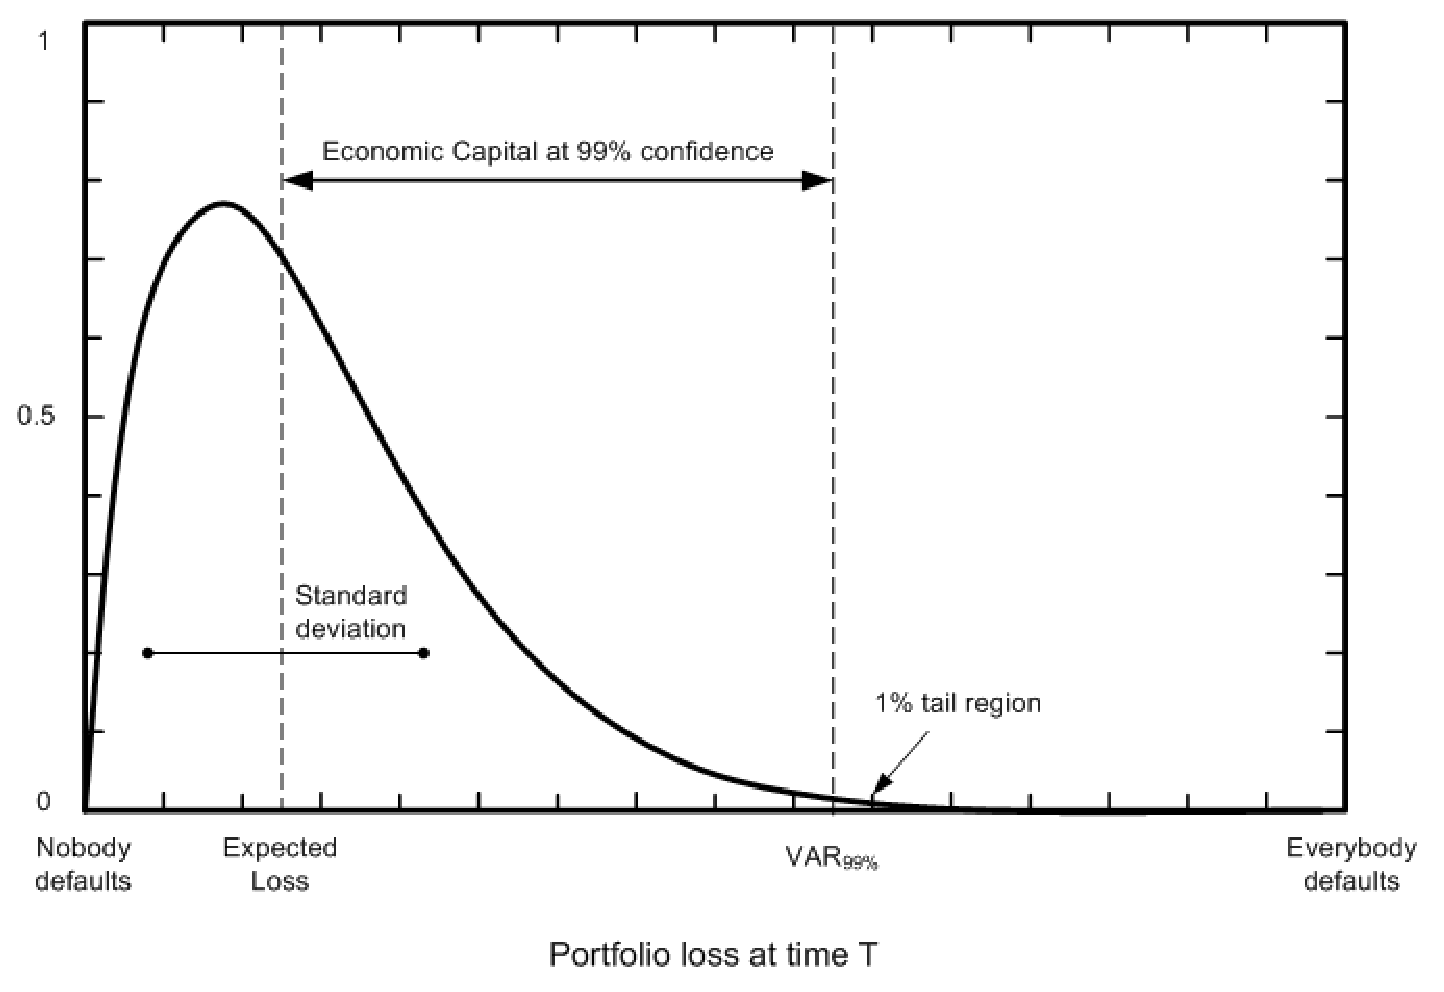
\includegraphics[height=7cm, angle=0]{./images/creditvar.eps}
\caption{Portfolio value at time $T$}
\label{creditvar}
\end{center}
\end{figure}

\paragraph{Ejemplo.} Intentemos calcular el VAR de una cartera de cr\'editos
sencilla, de la que se puede calcular la distribuci\'on de forma expl\'icita. 
Sea una cartera de $1$ solo sector con $100$ clientes sin correlaci\'on alguna
entre ellos. Cada cliente tiene un activo que consiste en devolver $1$ \euro al
cabo de $T$ tiempo. Supongamos que el sistema de ratings solamente contempla 
$2$ categor\'ias crediticias, no-Default y Default. La probabilidad de hacer 
fallido al cabo de $T$ tiempo es $0.1$.
\newline
\newline
En este caso, se puede modelar el importe devuelto por el cliente $i$ al cabo 
de $T$ tiempo como una variable aleatoria Bernouilli, $X_i \sim Ber(0.9)$. El 
valor de la cartera al cabo de $T$ tiempo es la suma de los importes devueltos 
por los clientes, $Y = \sum_{i=1}^{100} x_i$, que por definici\'on es una 
variable aleatoria Binomial, $Y \sim B(100,0.9)$. El Teorema Central del 
L\'imite nos permite aproximar $Y \sim B(100,0.9) \approx N(90, 9)$.
\newline
\newline
El valor esperado al cabo de $T$ tiempo es $E(Y) \approx 90$. Calculemos el VAR 
al nivel de confianza $99\%$:

\begin{displaymath}
\begin{array}{c}
P(Y \leq \textrm{VAR}_{99\%}) = 0.01 = 1\% \cr
P(90 + 3 \cdot X \leq \textrm{VAR}_{99\%}) = 0.01 \cr
P(X \leq \frac{\textrm{VAR}_{99\%} - 90}{3}) = 0.01 \longrightarrow \cr
\frac{\textrm{VAR}_{99\%} - 90}{3} = -2.33 \cr
\textrm{VAR}_{99\%} = -2.33 \cdot 3 + 90 = 83.01
\end{array}
\end{displaymath}
\newline
\newline
Este ejemplo no es significativo debido a que se han realizado dos supuestos 
que en el mundo real no se cumplen: todos los creditores se modelan de la misma 
forma y los fallidos son independientes. Se obtiene que la distribuci\'on del 
valor de la cartera a tiempo $T$ se aproxima a una variable aleatoria Normal,
cosa que no concuerda con las observaciones reales, que muestran que la
distribuci\'on del valor de las carteras es fuertemente asim\'etrica respecto
el valor esperado.

